%追加すべき事項
% - "音楽の表現"における音声処理の補強
% - "音楽の表現"の式(理解が必要)
% - "音楽の表現"の具体例(論文,既存研究)
% - "音楽の表現"の図
% - "音楽の表現"の単語の説明
\chapter{背景:音楽}

本章では、音の定義を行い、音の表現方法を紹介する。

\section{音の定義}

音とは、弾性体中を伝播する波により起こされる音波が聴覚により感じられるもののことである。

\subsection{音響信号}

音は時間方向の変化量であるため、音響信号と呼ばれる。音響信号は連続的な信号であるが、コンピュータで扱うために離散的な信号へと変換する必要がある。また、変換の際には標本化~(サンプリング)~と量子化が必要である。まず、サンプリングは一定の時間を空けて離散的に測定を行うことであり、1秒あたりのサンプリング回数をサンプリング周波数と呼ぶ。そして、量子化は信号の大きさを離散的に表現することであり、信号の大きさを表現するビット数を量子化ビット数と呼ぶ。

\subsection{楽音}

楽音は周期性のある音波を持つ音のことである。本論文では楽音としての音を生成することを目標とする。また、楽音は長さ、大きさ、高さ、音色の四要素を持つ。

\subsubsection{音の長さと大きさ}

音の長さは音波の時間長により決まり、音の大きさは音波の振幅により決まる~(\prettyref{fig:gakuon1})~。音波の時間長が長いほど音の長さは長くなり、音波の振幅が大きいほど音の大きさは大きい。

\subsubsection{音の高さと音色}

音の高さと音色は直感的にはそれぞれ音波の周期構造の長さと形により決まる~(\prettyref{fig:gakuon2})~。また、音の高さは音波の周波数により決まり、周波数の高い音ほど音の高さは高くなる。そして、音の長さと大きさと高さが同じ時の音の違いを音色と呼び、それぞれの楽器は異なる音色を持つ。

\begin{figure}[b]
\centering
\begin{minipage}{0.48\columnwidth}
\centering
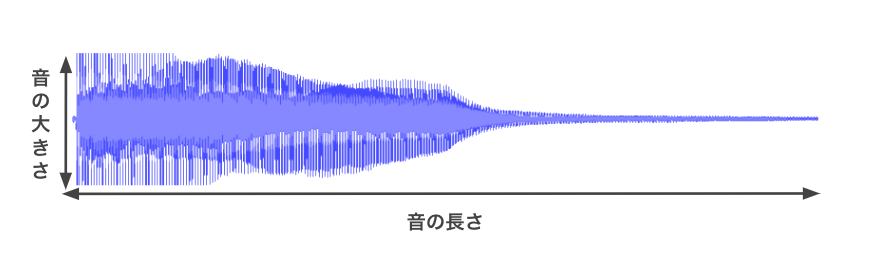
\includegraphics[width=\columnwidth]{figure/gakuon1.png}
\caption{音波}
\label{fig:gakuon1}
\end{minipage}
\begin{minipage}{0.48\columnwidth}
\centering
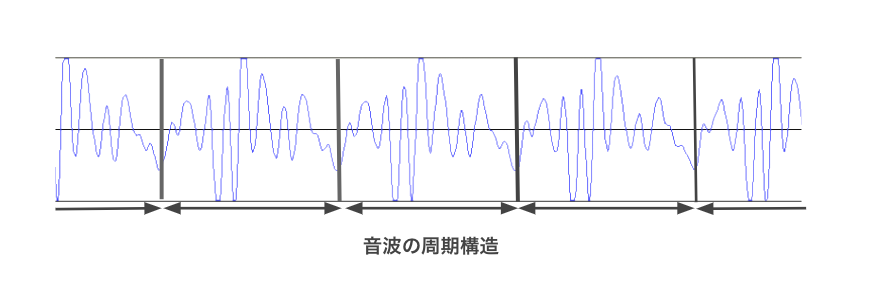
\includegraphics[width=\columnwidth]{figure/gakuon2.png}
\caption{音波の拡大図}
\label{fig:gakuon2}
\end{minipage}
\end{figure}

%ここで改ページ
\clearpage

\section{音の表現}

音をニューラルネットワークで扱うためには、楽音としての特徴を学習するための適切な表現を得る必要がある。また、本節は~\cite{musictutorial}及び~\cite{DL_ASP}を参考に作成し、本節の図は~\cite{musictutorial}のFigure~4と~\cite{timbretron}のFigure~2を利用している。

\subsection{一次元データと二次元データ}

素朴で連続的な音の表現である音響信号は離散的な一次元データへと変換される~(\prettyref{fig:audio_signal})~。音響信号は〇〇などの研究で△△という長所を利用されるが、ニューラルネットワークが楽音としての特徴を学習するには多くのデータが必要になると考えられる。

したがって、次節以降で紹介する二次元データへと変換して扱うことが一般的である。音響信号を周波数成分ごとに分解する操作により、次元としては時間と周波数を選ぶことが多い~(時間-周波数表現)~。また、この変換により音響信号の楽音としての特徴が明確化されるため、より効果的に特徴を学習できると考えられる。

\subsection{STFT}

STFT~(Short~Time~Fourier~Transform)~は時間-周波数表現を生成する基本的な手法であり、中間周波数を利用した線形間隔のバンドパスフィルターを用いて周波数成分を分解する。また、横軸を時間で縦軸を周波数とした画像をSTFTにより生成することができ、これをスペクトログラムと呼ぶ。ここで、STFTの具体的な計算方法については〇〇に詳しい。%勉強する

しかし、人間の聴覚系の周波数分解能は線形ではないかつ楽音の解析のために作成されたわけではないため、STFTのバンドパスは楽音の解析に適しているとは言えない。したがって、STFTはニューラルネットワークで扱う表現の作成において人気のある手法ではない。ただし、STFTは音源分離などに用いられることがある。%研究例を挙げる

\begin{figure}[b]
\centering
\begin{minipage}[b]{0.48\columnwidth}
\centering
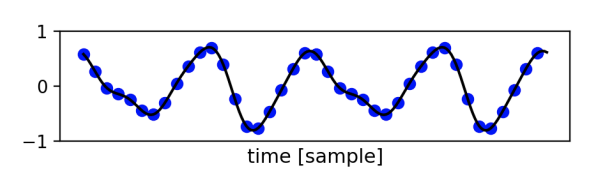
\includegraphics[width=\columnwidth]{figure/audio_signal.png}
\caption{音響信号}
\label{fig:audio_signal}
\end{minipage}
\begin{minipage}[b]{0.48\columnwidth}
\centering
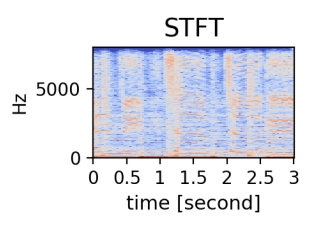
\includegraphics[width=\columnwidth]{figure/stft.png}
\caption{STFT}
\label{fig:STFT}
\end{minipage}
\end{figure}
    

%ここで改ページ
\clearpage

\subsection{メルスペクトログラム}

メルスペクトログラムはメル尺度~\cite{melscale}を用いてスペクトログラムにおいて周波数方向の圧縮を行ったものである。また、メル尺度は人間の感じる音の高さの差と差が等しくなるように調整した尺度であり、~\cite{mel}では周波数を$f$として\prettyref{eq:mel}のように定式化される。

\begin{align}
    \label{eq:mel}
    mel(f)=1127.01048\log{(\frac{f}{700}+1)}
\end{align}

メル尺度は人間の聴覚系に合わせた尺度であるため、スペクトログラムよりも楽音の解析に適している。また、経験的にもメルスペクトログラムは楽音のタスクに適していることが言える。%研究例

\subsection{CQT}

CQT~(Constant~Q~Transform)~は対数振幅の中心周波数を使用した二次元の表現である。CQTは対数振幅を用いており、音の高さの分布に近い。したがって、基音を正確に識別する際に用いられ、和音の識別や書き換えに使うことができる。

また、計算量としてはSTFTやメルスペクトログラムより重い。そして、単純な対数振幅のスペクトログラムが有効な例もある。

Rainbowgram,クロマも例

与えられた音の高さの集合におけるエネルギー分布のこと。多くの場合は西洋音楽の12音階をその集合とする。つまり、クロマグラムは周波数方向に畳み込んだCQTと見なすことができる。また、クロマグラムは他の表現方法よりも処理が進んだものなので、それ自身を特徴量として用いることができる。

\begin{figure}[b]
\centering
\begin{minipage}[b]{0.48\columnwidth}
\centering
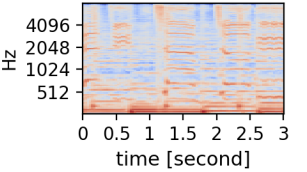
\includegraphics[width=\columnwidth]{figure/mel.png}
\caption{メルスペクトログラム}
\label{fig:mel}
\end{minipage}
\begin{minipage}[b]{0.48\columnwidth}
\centering
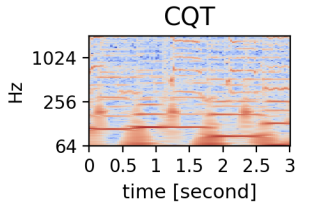
\includegraphics[width=\columnwidth]{figure/cqt.png}
\caption{CQT}
\label{fig:cqt}
\end{minipage}
\end{figure}
    